\subsection{Reading outside array bounds}

So, array indexing is just \IT{array\lbrack{}index\rbrack}.
If you study the generated code closely, you'll probably note the missing index bounds checking,
which could check \IT{if it is less than 20}.
What if the index is 20 or greater?
That's the one \CCpp feature it is often blamed for.

Here is a code that successfully compiles and works:

\lstinputlisting{patterns/13_arrays/2_BO/r.c}

Compilation results (MSVC 2008):

\lstinputlisting[caption=\NonOptimizing MSVC 2008]{patterns/13_arrays/2_BO/r_msvc.asm}

The code produced this result:

\begin{figure}[h]
\centering
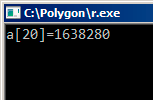
\includegraphics[scale=\NormalScale]{patterns/13_arrays/2_BO/olly_r3.png}
\caption{\olly: console output}
\label{fig:array_BO_olly_r3}
\end{figure}

It is just \IT{something} that was lying in the stack near to the array, 80 bytes away from its first element.

\clearpage
\myindex{\olly}
Let's try to find out where did this value come from, using \olly.

Let's load and find the value located right after the last array element:

\begin{figure}[H]
\centering
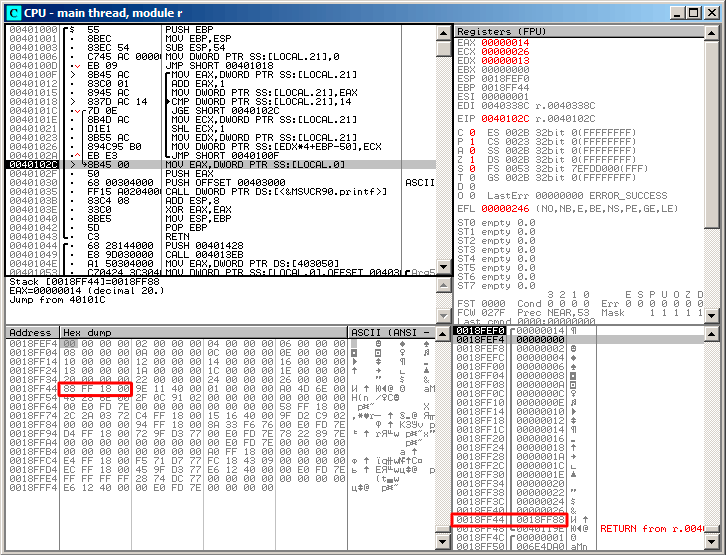
\includegraphics[scale=\FigScale]{patterns/13_arrays/2_BO/olly_r1.png}
\caption{\olly: reading of the 20th element and execution of \printf}
\label{fig:array_BO_olly_r1}
\end{figure}

What is this? 
Judging by the stack layout,
this is the saved value of the EBP register.
\clearpage
Let's trace further and see how it gets restored:

\begin{figure}[H]
\centering
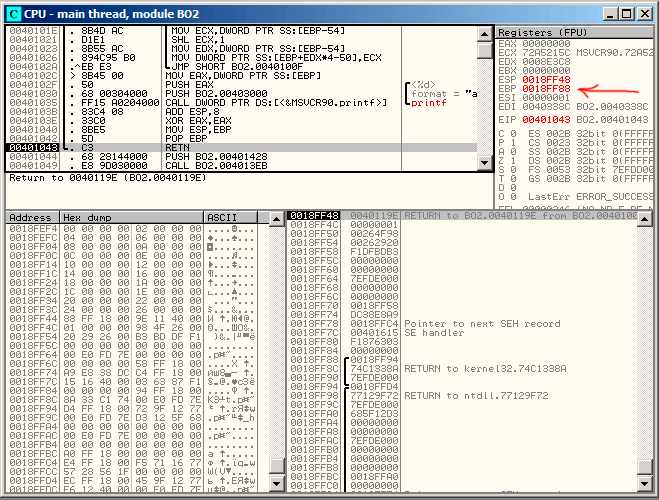
\includegraphics[scale=\FigScale]{patterns/13_arrays/2_BO/olly_r2.png}
\caption{\olly: restoring value of EBP}
\label{fig:array_BO_olly_r2}
\end{figure}

Indeed, how it could be different?
The compiler may generate some additional code to check the index value to be always
in the array's bounds (like in higher-level programming languages\footnote{Java, Python, etc})
but this makes the code slower.

